\documentclass[14pt]{extbook}
\usepackage{multicol, enumerate, enumitem, hyperref, color, soul, setspace, parskip, fancyhdr} %General Packages
\usepackage{amssymb, amsthm, amsmath, latexsym, units, mathtools} %Math Packages
\everymath{\displaystyle} %All math in Display Style
% Packages with additional options
\usepackage[headsep=0.5cm,headheight=12pt, left=1 in,right= 1 in,top= 1 in,bottom= 1 in]{geometry}
\usepackage[usenames,dvipsnames]{xcolor}
\usepackage{dashrule}  % Package to use the command below to create lines between items
\newcommand{\litem}[1]{\item#1\hspace*{-1cm}\rule{\textwidth}{0.4pt}}
\pagestyle{fancy}
\lhead{Progress Quiz 5}
\chead{}
\rhead{Version B}
\lfoot{8497-6012}
\cfoot{}
\rfoot{Summer C 2021}
\begin{document}

\begin{enumerate}
\litem{
Solve the equation below. Then, choose the interval that contains the solution.\[ -4(-10x -16) = -18(-12x -17) \]\begin{enumerate}[label=\Alph*.]
\item \( x \in [-1.52, -1.43] \)
\item \( x \in [-2.22, -2.09] \)
\item \( x \in [2.08, 2.11] \)
\item \( x \in [-1.44, -1.35] \)
\item \( \text{There are no real solutions.} \)

\end{enumerate} }
\litem{
Write the equation of the line in the graph below in Standard Form $Ax+By=C$. Then, choose the intervals that contain $A, B, \text{ and } C$.
\begin{center}
    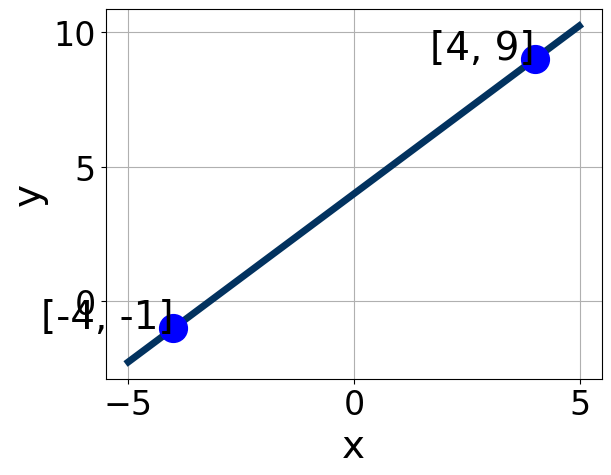
\includegraphics[width=0.5\textwidth]{../Figures/linearGraphToStandardCopyB.png}
\end{center}
\begin{enumerate}[label=\Alph*.]
\item \( A \in [-1.25, 0.75], \hspace{3mm} B \in [-0.2, 2.4], \text{ and } \hspace{3mm} C \in [3, 8] \)
\item \( A \in [-8, -4], \hspace{3mm} B \in [2.7, 5.5], \text{ and } \hspace{3mm} C \in [11, 22] \)
\item \( A \in [1, 6], \hspace{3mm} B \in [2.7, 5.5], \text{ and } \hspace{3mm} C \in [11, 22] \)
\item \( A \in [-1.25, 0.75], \hspace{3mm} B \in [-2.5, -0.3], \text{ and } \hspace{3mm} C \in [-12, 0] \)
\item \( A \in [1, 6], \hspace{3mm} B \in [-4.5, -1.8], \text{ and } \hspace{3mm} C \in [-18, -14] \)

\end{enumerate} }
\litem{
Solve the equation below. Then, choose the interval that contains the solution.\[ -7(-15x -6) = -10(14x -12) \]\begin{enumerate}[label=\Alph*.]
\item \( x \in [4.03, 4.99] \)
\item \( x \in [0.33, 1.74] \)
\item \( x \in [0.15, 0.49] \)
\item \( x \in [-1.36, 0.03] \)
\item \( \text{There are no real solutions.} \)

\end{enumerate} }
\litem{
Solve the linear equation below. Then, choose the interval that contains the solution.\[ \frac{5x + 9}{3} - \frac{3x + 5}{4} = \frac{-3x -7}{7} \]\begin{enumerate}[label=\Alph*.]
\item \( x \in [-3.5, -1.6] \)
\item \( x \in [-8.5, -6.2] \)
\item \( x \in [-4.3, -2.9] \)
\item \( x \in [-0.8, 0.5] \)
\item \( \text{There are no real solutions.} \)

\end{enumerate} }
\litem{
First, find the equation of the line containing the two points below. Then, write the equation in the form $ y=mx+b $ and choose the intervals that contain $m$ and $b$.\[ (8, -11) \text{ and } (-8, 2) \]\begin{enumerate}[label=\Alph*.]
\item \( m \in [-3.4, 0.6] \hspace*{3mm} b \in [9.3, 13] \)
\item \( m \in [-3.4, 0.6] \hspace*{3mm} b \in [-20.9, -17.2] \)
\item \( m \in [-0.2, 1.5] \hspace*{3mm} b \in [8.1, 9.3] \)
\item \( m \in [-3.4, 0.6] \hspace*{3mm} b \in [-5.4, -3.6] \)
\item \( m \in [-3.4, 0.6] \hspace*{3mm} b \in [3.1, 6.9] \)

\end{enumerate} }
\litem{
Find the equation of the line described below. Write the linear equation in the form $ y=mx+b $ and choose the intervals that contain $m$ and $b$.\[ \text{Perpendicular to } 7 x + 3 y = 6 \text{ and passing through the point } (-7, -10). \]\begin{enumerate}[label=\Alph*.]
\item \( m \in [-1.46, 0.06] \hspace*{3mm} b \in [-14, -9] \)
\item \( m \in [2.21, 2.76] \hspace*{3mm} b \in [-9, -6] \)
\item \( m \in [-0.33, 0.86] \hspace*{3mm} b \in [3, 12] \)
\item \( m \in [-0.33, 0.86] \hspace*{3mm} b \in [-4, -1] \)
\item \( m \in [-0.33, 0.86] \hspace*{3mm} b \in [-9, -6] \)

\end{enumerate} }
\litem{
Solve the linear equation below. Then, choose the interval that contains the solution.\[ \frac{7x + 5}{7} - \frac{3x -5}{2} = \frac{-6x + 4}{3} \]\begin{enumerate}[label=\Alph*.]
\item \( x \in [-0.83, 0.28] \)
\item \( x \in [-4.45, -3.37] \)
\item \( x \in [-1.47, -0.74] \)
\item \( x \in [1.6, 2.53] \)
\item \( \text{There are no real solutions.} \)

\end{enumerate} }
\litem{
First, find the equation of the line containing the two points below. Then, write the equation in the form $ y=mx+b $ and choose the intervals that contain $m$ and $b$.\[ (3, -8) \text{ and } (-11, -9) \]\begin{enumerate}[label=\Alph*.]
\item \( m \in [-0.02, 0.13] \hspace*{3mm} b \in [1, 4.9] \)
\item \( m \in [-0.33, -0.03] \hspace*{3mm} b \in [-10, -8.8] \)
\item \( m \in [-0.02, 0.13] \hspace*{3mm} b \in [-12.8, -9.8] \)
\item \( m \in [-0.02, 0.13] \hspace*{3mm} b \in [6.8, 11.1] \)
\item \( m \in [-0.02, 0.13] \hspace*{3mm} b \in [-8.5, -7.6] \)

\end{enumerate} }
\litem{
Write the equation of the line in the graph below in Standard Form $Ax+By=C$. Then, choose the intervals that contain $A, B, \text{ and } C$.
\begin{center}
    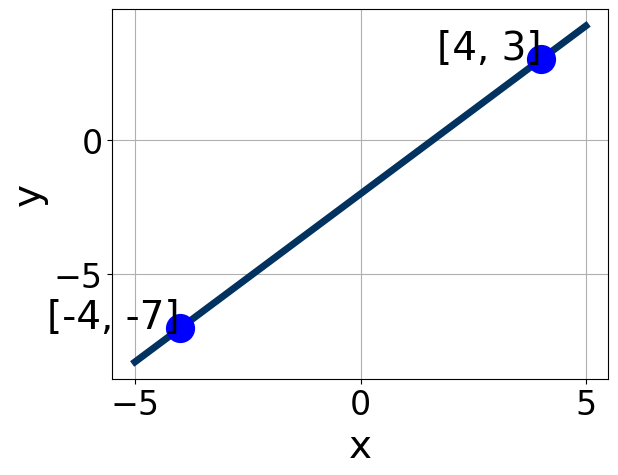
\includegraphics[width=0.5\textwidth]{../Figures/linearGraphToStandardB.png}
\end{center}
\begin{enumerate}[label=\Alph*.]
\item \( A \in [4.7, 7.3], \hspace{3mm} B \in [-6.8, -1.8], \text{ and } \hspace{3mm} C \in [6, 11] \)
\item \( A \in [-6, -2.5], \hspace{3mm} B \in [1.9, 4.5], \text{ and } \hspace{3mm} C \in [-12, -6] \)
\item \( A \in [-1.4, -0.9], \hspace{3mm} B \in [-0.7, 3], \text{ and } \hspace{3mm} C \in [-4, 1] \)
\item \( A \in [4.7, 7.3], \hspace{3mm} B \in [1.9, 4.5], \text{ and } \hspace{3mm} C \in [-12, -6] \)
\item \( A \in [-1.4, -0.9], \hspace{3mm} B \in [-3.4, -0.2], \text{ and } \hspace{3mm} C \in [2, 5] \)

\end{enumerate} }
\litem{
Find the equation of the line described below. Write the linear equation in the form $ y=mx+b $ and choose the intervals that contain $m$ and $b$.\[ \text{Parallel to } 8 x - 3 y = 8 \text{ and passing through the point } (8, -5). \]\begin{enumerate}[label=\Alph*.]
\item \( m \in [-1.4, 2.2] \hspace*{3mm} b \in [-28.33, -20.33] \)
\item \( m \in [1.8, 3.7] \hspace*{3mm} b \in [-14, -9] \)
\item \( m \in [1.8, 3.7] \hspace*{3mm} b \in [24.33, 27.33] \)
\item \( m \in [-3, -0.6] \hspace*{3mm} b \in [14.33, 21.33] \)
\item \( m \in [1.8, 3.7] \hspace*{3mm} b \in [-28.33, -20.33] \)

\end{enumerate} }
\end{enumerate}

\end{document}